\documentclass[04.3_buildingProcess.tex]{subfiles}
\begin{document}
    \subsubsection{Conductive Ink Process}
    \begin{flushleft}
        \noindent
        In addition to this, we tested the conductive ink on the wood and if there is 
        still enough conductivity. The result is that the microcontroller can notice a 
        change; however, the resistance was between 1.7k\si{\ohm} and 12.2M\si{\ohm} , 
        so we had to use an analog pin and a threshold to find out if a leave coupe is 
        connected (see Figure \ref{fig:leaveConductiveInk}).

        \begin{figure}[h!]
            \centering
            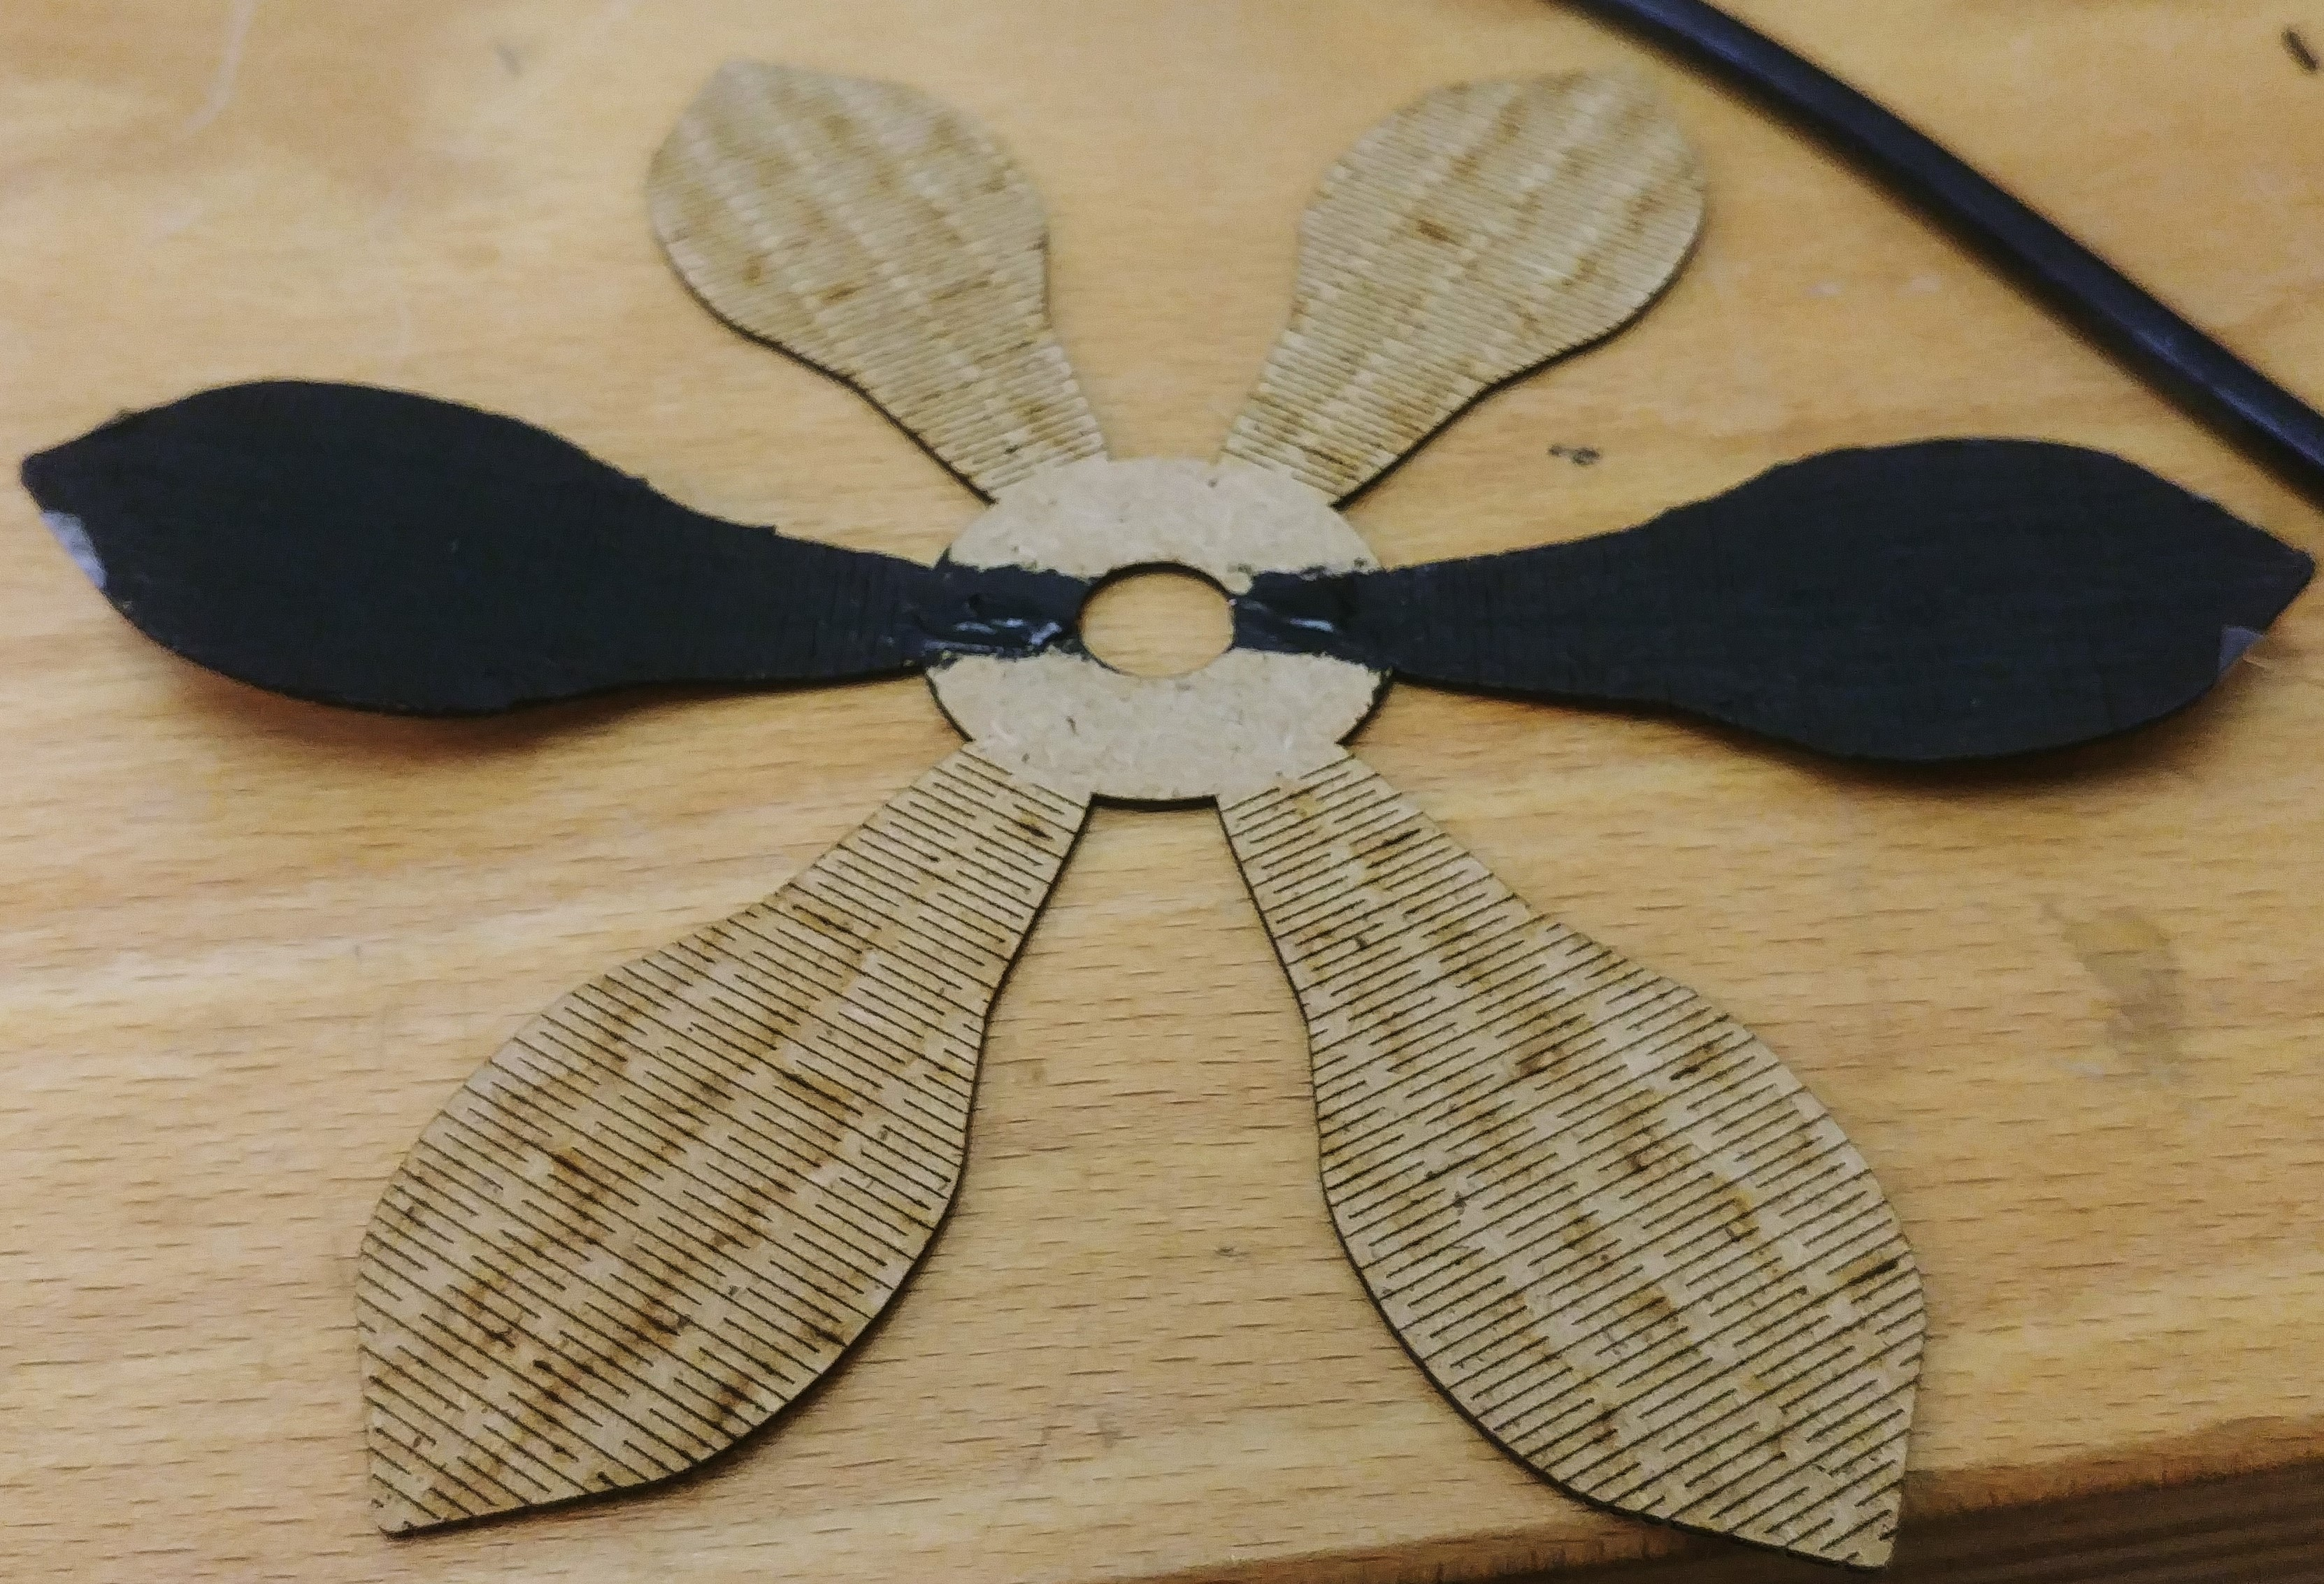
\includegraphics[scale=0.05]{images/materialProcess/leaveTesting_.jpg}
            \caption{Shows the testing of the conductive ink with wood.}
            \label{fig:leaveConductiveInk}
        \end{figure}

        \noindent
        After the conductive test (see Figure \ref{fig:leaveConductiveInk}), we wanted to paint 
        conductive ink on wood before laser cutting. Before, we asked the company if there is 
        something inside the paint that burns or is toxic. After knowing that it should be fine to 
        use the paint and later cut it. Therefore, we had to do some changes in the cutting pattern
        because the ink burns a bit stronger than the wood itself, so it burned parts of the leaves. 
        That's why we had to increase the distance between the cuts (see Figure \ref{fig:07_LaserCut}). 

        \begin{figure}[h!]
            \centering
            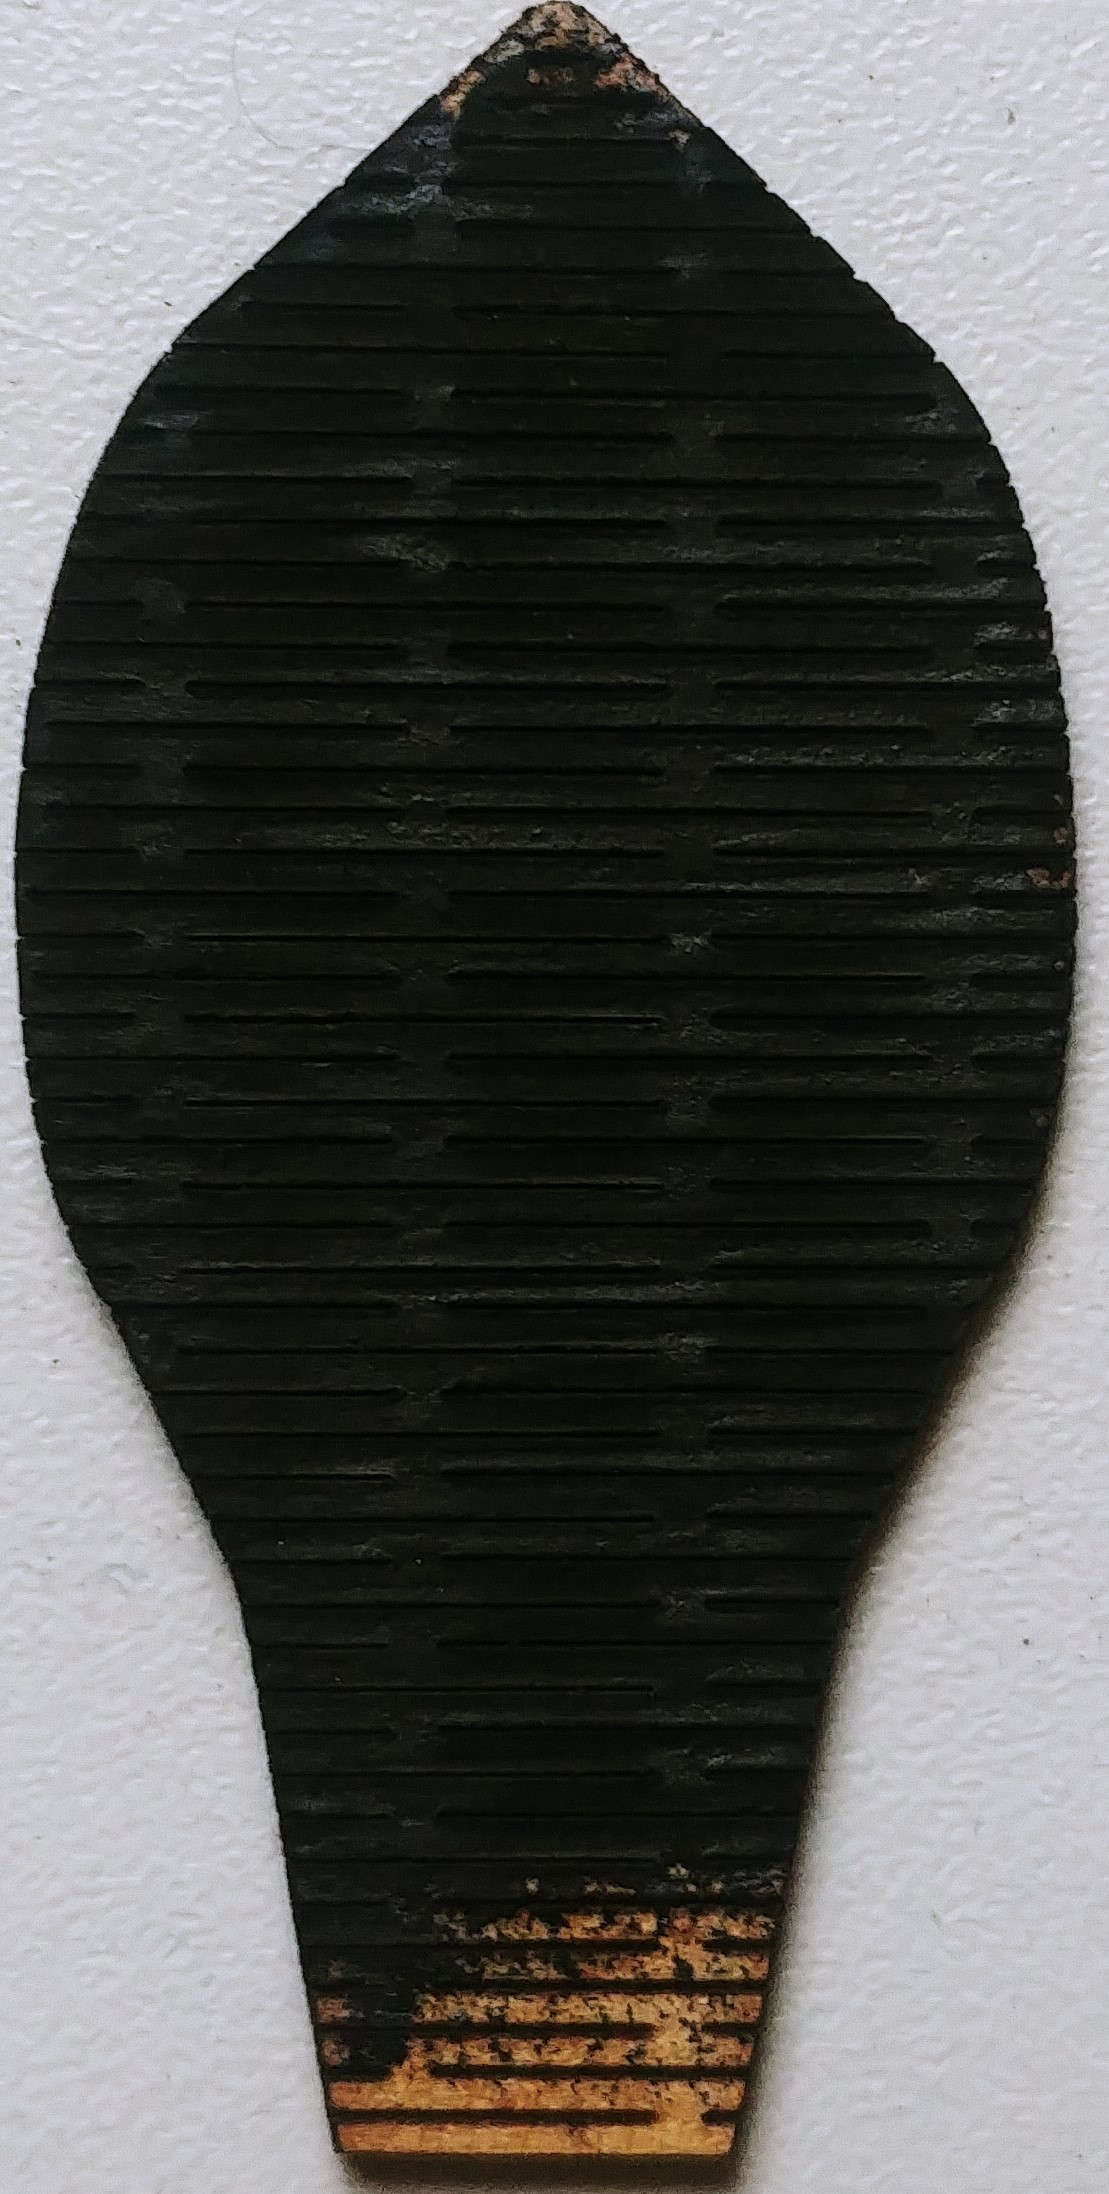
\includegraphics[scale=0.05]{images/materialProcess/07_LaserCut.jpg}
            \caption{Shows the result of the laser cut with capacitive ink on wood.}
            \label{fig:07_LaserCut}
        \end{figure}

        \noindent
        However, even after this success of cutting a test shape with a conductive ink, we couldn't 
        increase flexibility without increasing the size of the shape. However, we had to increase 
        the flexibility somehow because of the LEDs in the middle of the base and the light ball. 
        The diameter of the light ball is 3 centimeters. The flexibility and the size of the blossom 
        shape have to be large, so the leaves can connect and the not break. This problem couldn't 
        be solved in time, so we work with cork instead. This material is very flexiable, even 
        without cuts (see Figure \ref{fig:corkTest}).\\

        \begin{figure}[H]
            \centering
                \includegraphics[scale=0.05]{images/materialProcess/corkBlossomShape.jpg}
                \caption{Shows the corc blossom shape cut that will be used for the final prototype.}
                \label{fig:corkTest}
        \end{figure}
    \end{flushleft}
\end{document}